\chapter{Сэдвийн ерөнхий судалгаа}

Сэдвийн хүрээнд өмнө нь ажиллаж үзээгүй олон шинэ технологиудыг судалж хэд хэдэн шинэ технологи ашиглаж, тэдгээрийг үнэлж, харьцуулав. Энэ бүлэгт би судалгаанаасаа сонгосон технологиудыг танилцуулж, вэб платформыг бий болгох үндсэн ойлголтуудыг танилцуулж байна.

\section{Үндсэн ойлголтууд}

Энэхүү судалгааг амжилттай дуусгахын тулд зарим үндсэн ойлголтуудыг ойлгох нь зайлшгүй чухал юм.

\subsection{Web Sockets}

WebSocket нь хэрэглэгчийн хөтөч болон серверийн хооронд хоёр талын интерактив харилцааны session нээх боломжтой дэвшилтэт технологи юм. Энэхүү WebSocket - ийн тусламжтайгаар сервер рүү мэдээлэл илгээж, серверээс хариулт авах шаардлагагүйгээр үйл явдалд тулгуурласан хариултуудыг хүлээн авах боломжтой.

\begin{itemize}

	\item Real-time Interaction: Хэрэглэгчдийг бодит цаг хугацаанд бие биетэйгээ уралдуулахыг хүсвэл WebSockets маш чухал. Тэд оролцогч бүрийн мэдээллийг бусад бүх оролцогчдын дэлгэцэн дээр нэн даруй шинэчлэх боломжийг олгоно.
	\item Dynamic Updates: Хэрэв тоглоомын орчин, дүрэм, зард ямар нэгэн өөрчлөлт орсон бол WebSockets нь бүх идэвхтэй хэрэглэгчдэд шууд мэдэгдэх боломжтой
	\item Multiplayer Racing: Олон оролцогчтой уралдааны хувьд тоглоомын төлөвийг удирдаж, хэрэглэгчдэд синхрончлолыг хангах нь WebSockets-ийн тусламжтай илүү удирдах боломжтой болно.
\end{itemize}

WebSockets нь бодит цагийн интерактив платформын салшгүй технологийн нэг бөгөөд шуурхай шинэчлэлт, харилцан үйлчлэлд шаардагдах хурд, үр ашгийг санал болгодогоороо давуу талтай.

\subsection{Web-based Educational Platforms}

Вэб дээр суурилсан платформууд нь хэрэглэгчид хүссэн үедээ, хаанаас ч, ихэвчлэн өөрийн хүссэн хэмжээгээр систем руу хандах боломжтойгоороо давуу талтай.

Өрсөлдөх чадвартай эсвэл хамтран ажиллах боломжуудыг агуулж, суралцахыг нийгмийн туршлагыг бий болгож хэрэглэгчид дэлхийн хэмжээнд үе тэнгийнхэнтэйгээ өрсөлдөх эсвэл тэднээс суралцах боломжтой.
\section{Ижил төсөөтэй систем}

\subsection{TypingTest.com}

"TypingTest Pro" нь хэрэглэгчид бичих хурд, нарийвчлалыг хэмжихэд зориулагдсан онлайн платформ юм. Энэ платформ нь хэрэглэгчдэд бодит цагийн горимд бичих янз бүрийн текстүүдийг өгч, гүйцэтгэлийн талаар шууд санал хүсэлтийг санал болгодог.

\begin{figure}[h]
	\centering
	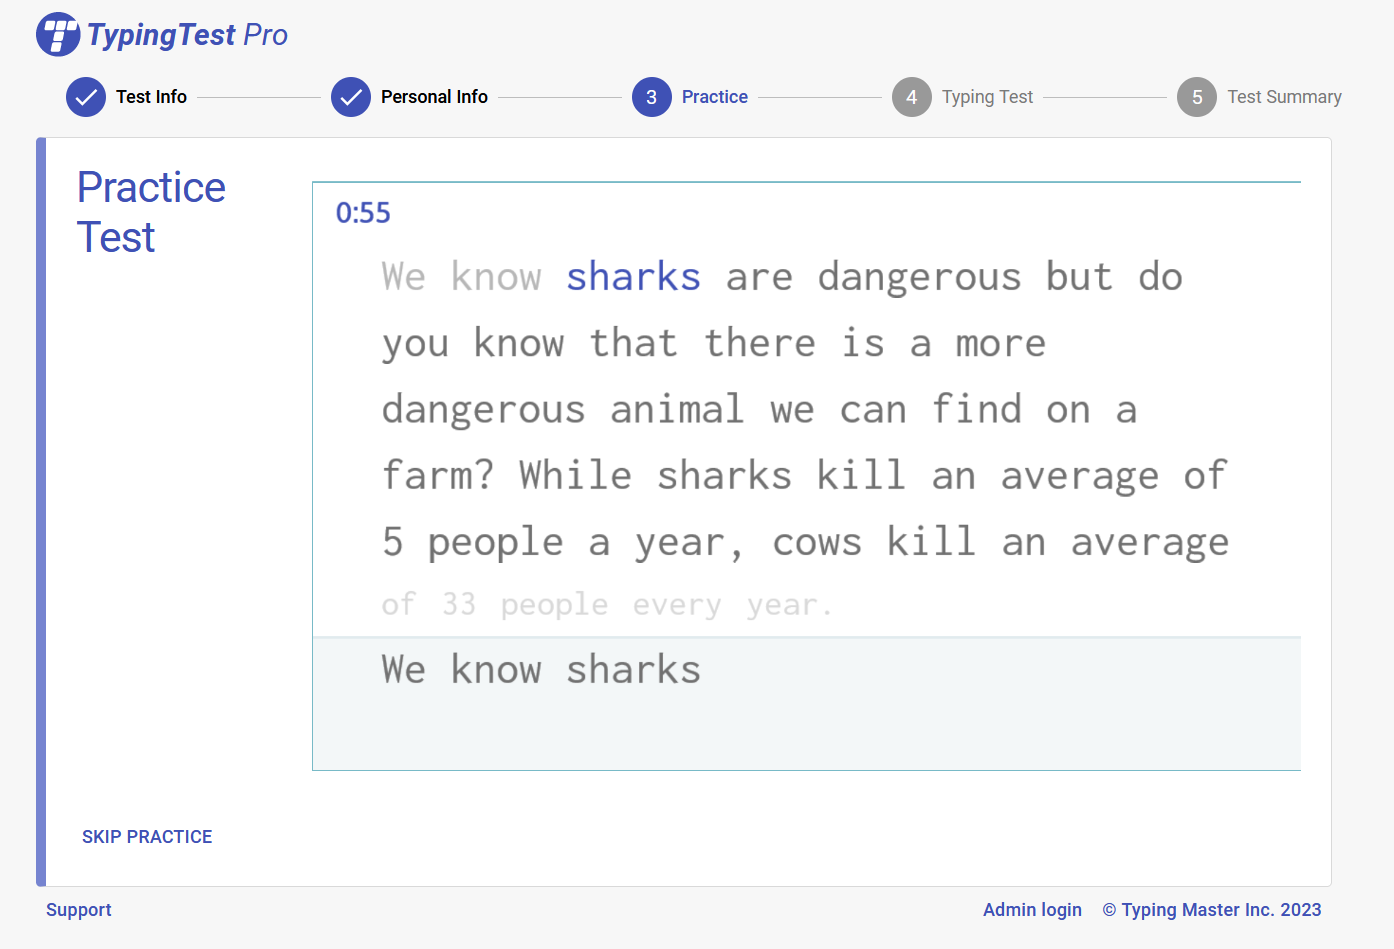
\includegraphics[width=15cm]{images/typingtestpro.png}
	\caption{typingtest.com/pro/ сайтын харагдах байдал}
	\label{fig:alltop}
\end{figure}

Манай бүтээх гэж байгаа вебээс ялгаатай тал нь
\begin{itemize}
	\item 1-ээс 10 минутын хугацаатай туршилтуудыг санал болгож, хэрэглэгчдэд сорилтын түвшингээ сонгох боломжийг олгодог.
	\item Шууд guest хэлбэрээр орон тест өгөх боломжгүй
\end{itemize}

Frontend: HTML5, CSS3 болон динамик хэрэглэгчийн интерфэйсүүдэд зориулсан React.js-тэй JavaScript.
Backend: Express.js хүрээтэй Node.js нь өргөтгөх боломжтой, үр ашигтай сервер талын програмыг хангадаг.
Өгөгдлийн сан: Хэрэглэгчийн профайл, тестийн үр дүн, текстийн хэсгүүдийг хадгалах MongoDB.WebSockets: Бодит цагийн өрсөлдөөн, шууд санал хүсэлтийн функцэд зориулагдсан.
Third-party Integrations: Дэлхий даяар тэргүүлэгчдийн самбар, олон нийтийн мэдээллийн хэрэгслээр хуваалцах боломжууд.

Онлайнаар шивэх тестийн олон платформууд байдаг ч "TypingTest Pro" нь энгийн хэрэглэгчид болон бичих чадвараа сайжруулахад нухацтай ханддаг хүмүүст зориулсан иж бүрэн функцээрээ бусдаас ялгардаг.

\subsection{play.typeracer.com}

TypeRacer бол олон тоглогчийн онлайн хөтөч дээр суурилсан шивэх тоглоом юм. Тоглогчид богино хэсгийг аль болох хурдан шивэх замаар өрсөлддөг бөгөөд тоглоом нь хурдыг минут тутамд үгээр (WPM) болон нарийвчлалыг хэмждэг. Үүсгэн байгуулагдсан цагаасаа эхлэн энэ нь өрсөлдөөнтэй, хөгжилтэй орчинд бичих чадвараа сайжруулахыг хүсч буй хүмүүсийн дуртай хэрэгсэл болсон.

\begin{figure}[h]
	\centering
	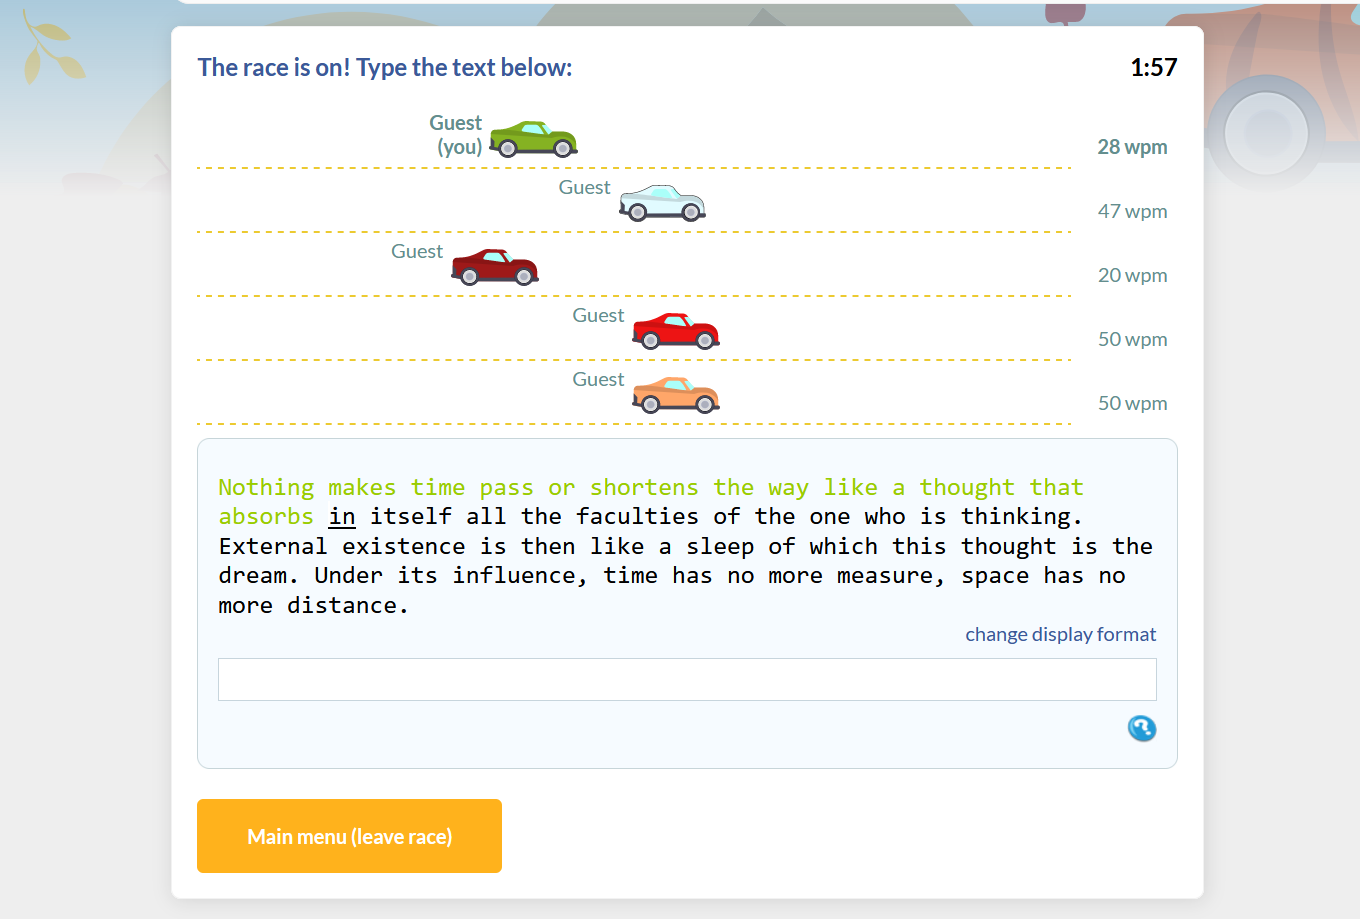
\includegraphics[width=15cm]{images/TypeRacer.png}
	\caption{play.typeracer.com сайтын харагдах байдал}
	\label{fig:linktree}
\end{figure}

Гол онцлог:

Энэ бол вэб дээрх анхны олон тоглогчийн шивэх тоглоом юм.

2008 оны 3-р сард нээлтээ хийснээс хойш дэлхийн өнцөг булан бүрээс сая сая хүмүүс typeracer.com сайт дээр хэдэн зуун сая уралдаанд оролцож, бичих хурдаа минут тутамд 50 үгээр сайжруулсан.

TypeRacer нь 50 өөр хэл дээр байдаг.

2010 онд гарсан TypeRacer School Edition нь дэлхийн хамгийн хөгжилтэй боловсролын бүтээгдэхүүн болох зорилготой юм. K-12 сургуулиудад зориулагдсан бөгөөд бичихийг спорт болгон хувиргаж, суралцахыг хөгжилтэй болгодог TypeRacer тоглоомын үзэл баримтлалыг ашигладаг.
% \section{Ашиглах технологи}

\subsection{Figma - интерфейс дизайн, Prototype хувилбар гаргах багаж}
Figma нь хэрэглэгчдэд нэг платформ дээр дизайн хийх, загвар гаргах, санал хүсэлтийг цуглуулах боломжийг олгодог хамтын дизайны хэрэгсэл юм. Дизайнерууд, хөгжүүлэгчид, бүтээгдэхүүний менежерүүд болон оролцогч талууд бодит цаг хугацаанд хамтран ажиллах боломжтой бөгөөд энэ нь дижитал бүтээгдэхүүн дээр ажилладаг багуудад хүчирхэг хэрэгсэл болгодог.

Figma ашиглахын давуу талууд
\begin{itemize}
	\item Вэб дээр суурилсан бөгөөд энэ нь том хэмжээний програм хангамжийн багц татаж авах шаардлагагүй. Windows, MacOS, Linux зэрэг өөр өөр үйлдлийн системүүд дээр саадгүй ажилладаг
	\item Хийсэн өөрчлөлтүүдийг автоматаар хадгалж, шаардлагатай бол хуучин өөрчлөлт рүү буцах боломжийг олгодог
	\item Figma нь оюутнуудад нэмэлт зардал гаргахгүйгээр иж бүрэн төсөл хэрэгжүүлэх боломжийг үнэ төлбөргүй санал болгодог.
\end{itemize}

% \begin{figure}[h]
% 	\centering
% 	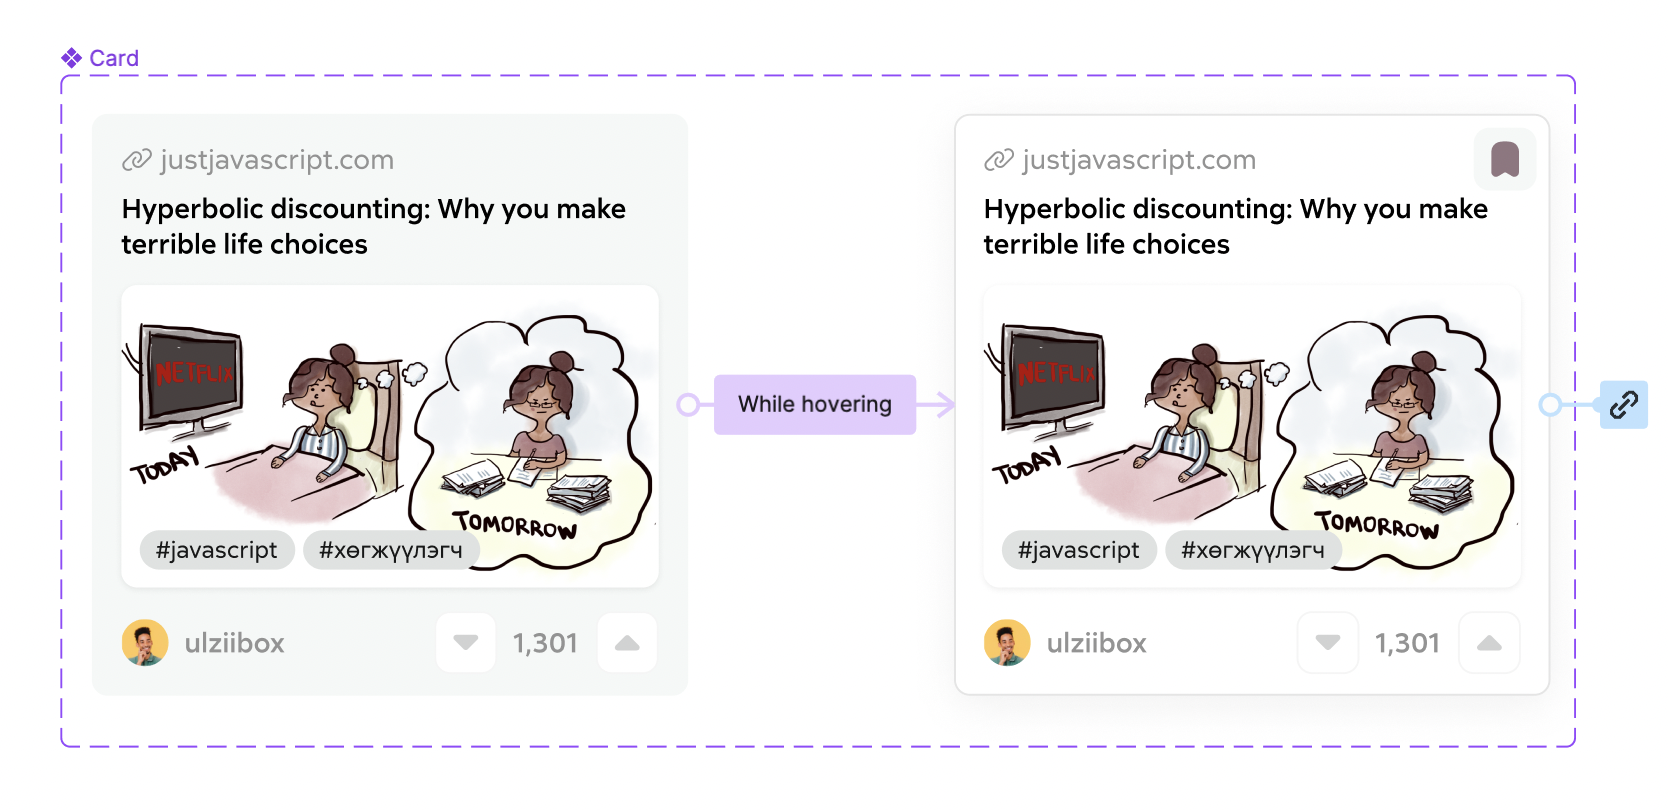
\includegraphics[width=10cm]{images/figma-prototype.png}
% 	\caption{Figma ашиглаж Card-н hover эффект дээр prototype хийсэн компонент}
% 	\label{fig:figma}
% \end{figure}

Зурсан интерфейсүүдээ хооронд нь холбож хийсвэрээр аппаа ажиллуулан хэрэглэгчийн туршилт хийх хэсгийг Prototype гэдэг бөгөөд заавал кодын хэрэгжүүлэлт хийж цаг хугацаа болон мөнгөн зардал гаргалгүйгээр хийж буй аппаа хэрэглэгчээр туршуулах, үр дүнгээ гарган авч түүнийгээ сайжруулах нөхцөлийг уг веб аппликейшн маань гаргаж өгсөн нь UX/UI дизайнеруудын ашиглах болсон хамгийн том шалтгаануудын нэг юм.
\subsection{React - Javascript сан}

\subsubsection{Сонгосон шалтгаан}

Хэдийгээр олон төрлийн технологи ашиглан уг бүтээгдэхүүнийг хөгжүүлэх боломжтой ч орчин үед хамгийн трэнд болж буй уг технологийн тусгайлан сонгож аван судалж үзлээ. Хамгийн эхлээд 2023 онд хамгийн ихээр ашиглаж буй вэб фрэймворкийн судалгааг \footnote{Вэб фрэймворкийн судалгаа \url{https://www.knowledgehut.com/blog/web-development/front-end-development-frameworks}} танилцуулъя.

\begin{figure}[h]
	\centering
	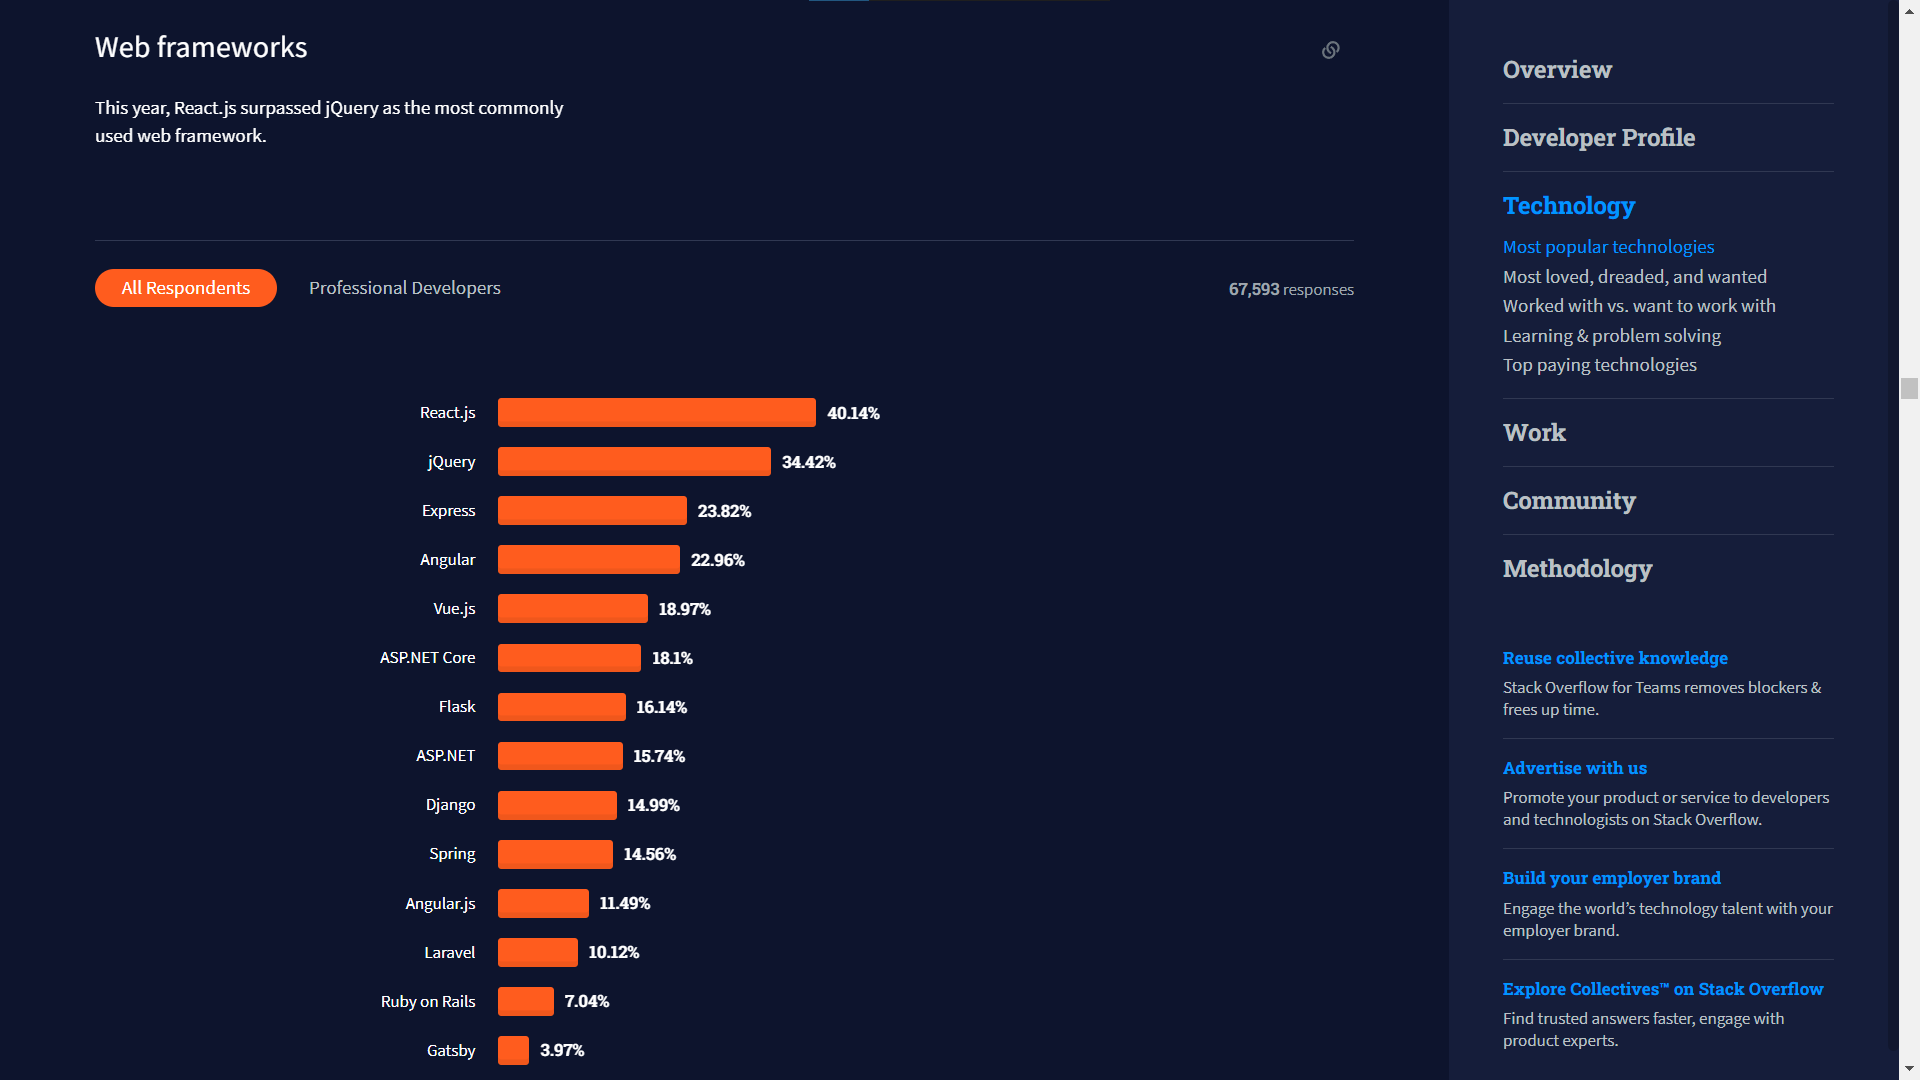
\includegraphics[width=12cm]{images/most-used-frameworks.png}
	\caption{2022 онд хамгийн ихээр ашиглаж буй вэб фрэймворкийн жагсаалт}
	\label{fig:most-used-frameworks}
\end{figure}

Энэ судалгаанаас та React.js-г вэбийн Front-End хэсэг дээр хамгийн ихээр ашиглаж буйг харж болно.

Мөн Javascript хэл ашиглан хийсэн, хөгжүүлэлт хийхэд хялбар, client болон server-side аппликейшн хийх боломжтой, виртуал DOM гэсэн ойлголтыг оруулж ирснээр бусад сангуудаас илүү хурдан ажиллах боломжийг олгосон нь уг санг сонгосон хамгийн том шалтгаанууд юм.

\subsubsection{Технологийн талаар}

Фэйсбүүк компани дотооддоо ашиглаж байсан технологио 2013 онд танилцуулсан нь програмчлалын Javascript хэлийг ашиглаж хийсэн Front-end library болох React\footnote{Reactjs official site \url{https://reactjs.org}} технологи юм. Declarative UI хөгжүүлэлтийн аргыг хамгийн анх дэлгэрүүлж, өргөн хэрэглээнд нэвтрүүлж чадсан тул Declarative UI-н гол төлөөлөгч гэж явдаг. Уг технологийг ашиглахын тулд үндсэн хэдэн ойлголтууд авах хэрэгтэй. Үүнд component ба түүний lifecycle, javascript-н өргөжүүлсэн хувилбар болох jsx, мөн хамгийн чухал зүйл болох Virtual DOM нар багтана.

Declarative UI гэдэг нь хэрэглэгчийн интерфейсийн кодыг бичихдээ юу зурагдах буюу render хийх үеийн интерфейсийг бүгдийг урьдчилан тодорхойлдог арга барил юм. Imperative програмчлалаас ялгаатай нь хязгаартай нөхцөлд яг юу хийхийг хатуугаар зааж өгөхгүйгээр тухайн state-с хамааруулж хэрэглэгчийн хүссэн зүйлийг гаргаж өгөх боломжтой.

React нь component-based буюу DOM дээр хэвлэж байгаа бүх зүйлс component байна гэсэн дүрмийг баримталдаг. Component үүсгэж бичихийн давуу тал нь нэг бичсэн кодоо олон дахин бичигдэхээс зайлсхийж, дахин ашиглах боломжийг олгодог. Тус бур өөрсдийн гэсэн дотоод төлөвтэй мөн гаднаас утга хүлээн авах чадвартай. Үүнийг бид Props гэж нэрлэдэг. Мөн component нь stateless, stateful гэж хоёр хуваагддаг ба stateful component нь өөрийн гэсэн төлөвтэй, түүнийгээ удирддаг, class болон hook ашигласан функцууд байна. React-н давуу тал нь state эсвэл props-н өөрчлөлтийг үргэлж хянаж байдаг тул өөрчлөлт орж ирэхэд бүтэн хуудсыг зурах бус зөвхөн тухайн өөрчлөгдсөн component-г л дахин зурдаг. Ингэснээр энгийн вебүүдээс илүү хурдтай ажилладаг.

\begin{lstlisting}[language=Javascript, caption=JSX ашиглаж 'container' класстай html элемент буцаах компонент, frame=single]
	export function Container = ({children}) => {
		return (
			<div className="container">
				{children}
			</div>
		)
	}
			
\end{lstlisting}

JSX нь Javascript Extended гэсэн үгний товчлол бөгөөд энгийнээр javascript дотор HTML-н тагуудыг бичиж өгөх мөн кодыг илүү богино болгож хүссэн үр дүндээ хүрэх боломжийг олгодог. Үүний цаана Babel гэсэн transcompiler-г ашиглаж дундын хөрвүүлэлтийг хийдэг ба хэдийгээр HTML таг бичиж байгаа харагддаг ч код дунд цэвэр HTML-г огтоос бичиж өгдөггүй гэсэн үг юм \footnote{Дадлагын хугацаандаа хийж байсан технологийн судалгаанаасаа иш татав \url{https://github.com/ulziibox/intern-report/blob/main/main.pdf}}.

\subsection{Next.js - React дээр суурилсан фрэймворк}

\subsubsection{Сонгосон шалтгаан}

Reactjs өөрийг нь ашиглаж төсөл эхлүүлэхэд router, хуудаслалтаас эхлээд олон төрлийн тохиргоо хийх шаардлагатай болдог нь хөгжүүлэлтийн цагийг их үрдэг. Харин Next.js фрэймворк нь тэр бүх тохиргоог нэг л коммандаар хийж, зөвхөн код дээрээ анхаарал хандуулах боломжийг олгодог нь давуу талтай. Тэгэхээр дан Reactjs дээр төслөө эхлүүлсний оронд фрэймворк ашигласан нь хөгжүүлэлтийн хурдад эерэгээр нөлөөлнө гэж үзлээ. 

Next.js давуу талуудаас дурьдвал:
\begin{itemize}
	\item Image Optimization буюу их хэмжээтэй зураг оруулахад автоматаар зургийн чанарыг алдагдалгүйгээр хэмжээг багасгаж өгдөг
	\item Zero config буюу нэг ч тохиргоо хийлгүйгээр төслөө эхлүүлэх боломж
	\item Static Site Generator болон Server Side Render хийх
	\item Typescript болон Fast Refresh дэмждэг
	\item File-system Routing буюу “pages” гэсэн хавтас дотор үүссэн файлуудаас хамаарч вебийн замууд тодорхойлогддог мөн dynamic routing ашиглах боломжтой
	\item API Routes буюу өөр дээрээ nodejs сервер ашиглаж API endpoint гаргах боломжтой. Ингэснээр тусдаа сервер ашиглах шаардлага үүсэхгүй
	\item SEO буюу хайлтын системийн оновчлолыг SSR ашиглаж тохируулж өгөх гэх мэт маш олон давуу талуудтай
\end{itemize}

Мөн ердөө ганц “build” командаар статик болон динамик вебийг гарган авч ямар нэгэн веб сервер /apache, nginx гэх мэт/ ашиглалгүйгээр сервер дээрээ шууд байршуулах боломжтой юм.

\subsubsection{Технологийн талаар}

Next.js\footnote{Next.js official site \url{https://nextjs.org}} нь React сан дээр суурилж хөгжүүлсэн нээлттэй эхийн фрэймворк бөгөөд Vercel компани 2016 онд албан ёсны танилцуулгаа хийж олон нийтэд зарласан юм. React нь зөвхөн хэрэглэгчийн интерфейсийг зурах үүрэгтэй сан ба бусад веб хөгжүүлэлтэд хэрэгтэй хуудас хооронд шилжих гэх мэт үйлдлийг react-router болон бусад маш олон нэмэлт сангаас сонголт хийж шийдэх шаардлагатай байсан нь төслийн эхлэх явцыг удаашруулах хандлагатай байдаг. Харин Next.js ашигласнаар нэг ч тохиргоо хийлгүйгээр төслийг эхлүүлж шууд код бичих боломжийг бүрдүүлдэг. Цаана нь хийгдсэн тохиргоо нь нийт вебсайтуудын 90 хувийн шаардлагыг хангаж чаддаг гэж үздэг нь уг фрэймворкын сүүлийн жилүүдэд эрэлттэй болж буй шалтгаануудыг нэг билээ.


% \subsection{PostgreSQL - Өгөгдлийн сан}

% Платформынхоо өгөгдлийн сан дээр ашиглахаар сонгосон PostgreSQL нь 20 жилийн турш идэвхтэйгээр нээлттэй эхээр хөгжүүлэгдэж ирсэн өгөгдлийн сан бөгөөд SQL болон JSON Query дэмждэгээрээ илүү давуу талтай юм. Мөн олон төрлийн ORM дэмжиж ажиллах боломжтой.

% Түүхийн хувьд 1986 онд Калифорнийн Их Сургуулийн Компьютерын Ухааны тэнхимд POSTGRES гэдэг нэртэйгээр төсөл нь эхэлжээ. PostgreSQL нь Linux, UNIX (AIX, BSD, HP-UX, SGI IRIX, Mac OS X, Solaris, Tru64) болон Windows үйлдлийн системүүд дээр ажилладгаас гадна Apple, Fujitsu, Red Hat, Cisco, Instagram гэх мэт томоохон компаниуд өөрсдийн зарим бүтээгдэхүүнийхээ технологийн шийдлийг уг өгөгдлийн сан дээр шийдсэн байна.

% \subsection{Prisma - Нээлттэй эхийн ORM}

% Prisma нь PostgreSQL, MySQL, SQL Server, SQLite болон MongoDB ашиглаж хурдан хугацаанд, алдаа багатай апп бүтээхэд зориулагдаж гарсан нээлттэй эхийн ORM (Object–relational mapping) юм. Нийт 3 хэсгээс бүрдэх ба үүнд

% \begin{enumerate}
% 	\item Prisma Client - Node.js болон Typescript хэл ашиглаж query бичих багаж
% 	\item Prisma Migrate - Prisma Cli, Prisma Scheme ашиглан migration хийх багаж
% 	\item Prisma Studio - GUI ашиглан өгөгдлийн сангаа харах, засвар боломжтой багажууд багтана.
% \end{enumerate}

% \begin{figure}[h]
% 	\centering
% 	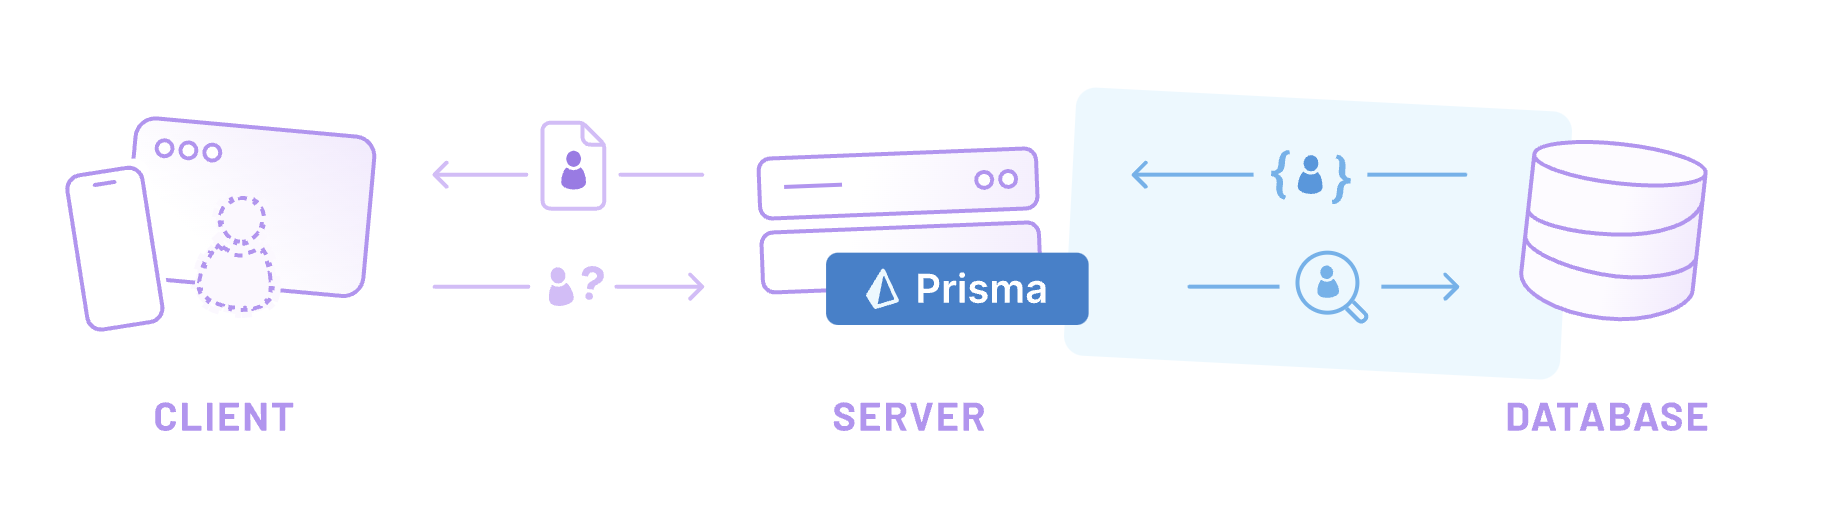
\includegraphics[width=15cm]{images/prisma-stack.png}
% 	\caption{Prisma тойм зураг}
% 	\label{fig:prisma}
% \end{figure}

% Уг технологийг сонгох болсон гол шалтгаан нь Next.js дээр back-end хөгжүүлэлтээ хийхэд Prisma ORM нь хамгийн тохиромжтой гэж үзсэнд ба SQL бичихгүйгээр өгөгдлийн сангаа удирдах боломжтой. Энэ нь миний хувьд илүү хурдан хугацаанд хангалттай үр дүнд хүрэх боломжийг өгч байна.